Android is an operating system (OS) developed by Google Inc.


\subsection{Android Architecture}
The Android platform is an open-source and Linux-based software stack, containing six major components [cite]: 

\begin{itemize}
    \item \verb|Applications|: Android provides a core set of applications (e.g., SMS, Mail, and browser) pre-installed on the device. There are support for installing third-party applications, which allows users to install applications developed by external vendors. A user is not bound to use the pre-installed applications for a service (e.g., SMS), and can choose the desired applications for a service. Also, third-party applications can invoke the functionality of the core applications (e.g., SMS), instead of developing the functionality from scratch. 
    \item \verb|Android Framework|: Is the building blocks to create Android applications by utilizing the core, all exposed through an API. The API enables reuse of core, modular system components, and services; briefly characterized as: \textit{View System}---to build the user interface pre-defined components (e.g., lists, grids, and buttons); \textit{Resource Manager}---provides access to resources (e.g., strings, graphics and layout files); \textit{Notification Managers}---allows applications to show custome notifications in the status bar; \textit{Activity Manager}---manages lifecycle of the application; and \textit{Content Providers}---enables applications to access data from other applications.
    \item \verb|Android Runtime|: Applications run its own process and has its own instance of the Android Runtime (ART). ART is designed to run on multiple virtual machines by executing DEX (Dalvik Executable format) files, which is a bytecode specifcally for Android to optimize memory footprint. Some of the features that ART provides are ahead-of-time (AOT) and just-in-time (JIT) compilation, garbage collection (GC), and debugging support (e.g., sampling profiler, diagnostic exceptions and crash reporting).
    \item \verb|Native Libraries|: Most of the core Android components and services native code, that requires native libraries, is written in C or C++. The Android platform exposes Java APIs to some of the functionality of the native libraries (with Android NDK).   
    \item \verb|Hardware Abstract Layer|: Provides an interface to expose hardware capabilities to the Java API framwork. Hardware Abstract Layer (HAL) consists of multiple library modules that implements an interface for specific hardware components (e.g., camera, or bluetooth module).
    \item \verb|Linux Kernel|: is the fundation of the Android platform. The ART relies on the functionality from the Linux kernal, such as threading and low-level memory management. The Linux kernel provides drivers to services (e.g., Bluetooth, Wifi, and IPC), and incorporates a component for power management. 
\end{itemize} 

\begin{figure}
    \centering
    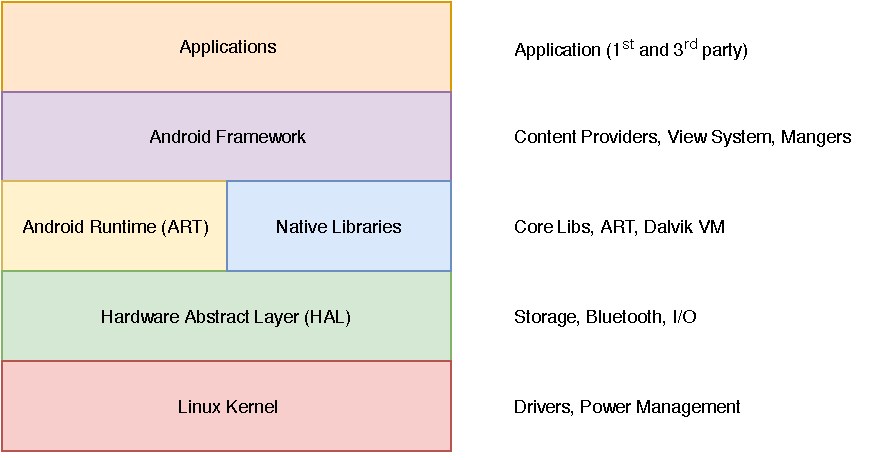
\includegraphics[scale=0.85]{images/Android.pdf}
    \caption{Recording}
    \label{fig:hta_recording}
\end{figure}

\subsection{Application Components}
\subsubsection{Activity \& Fragments}

\begin{figure}
    \centering
    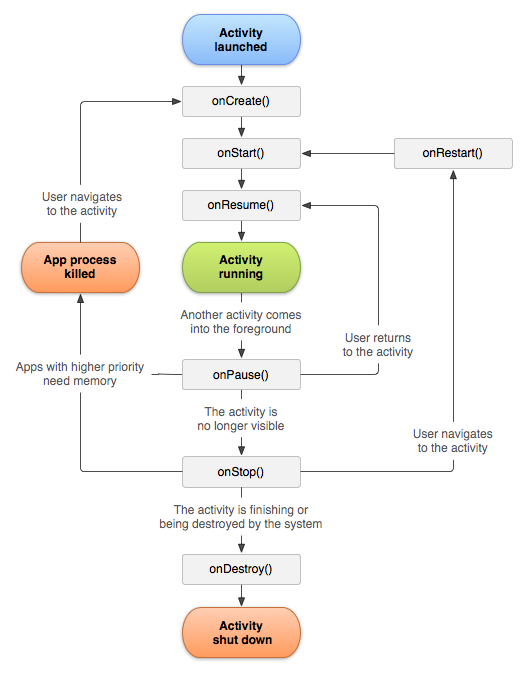
\includegraphics[scale=0.6]{images/androidlifecycle.png}
    \caption{Recording}
    \label{fig:hta_recording}
\end{figure}

\subsubsection{Service}
\subsubsection{Broadcast Reciver}

\subsection{Process and Threads}

\subsection{Inter-Process Communication}

\subsection{Bluetooth LE}

\subsection{Architecture Patterns}


\subsection{Energy Saving}